%%
% Please see https://bitbucket.org/rivanvx/beamer/wiki/Home for obtaining beamer.
%%
\documentclass[handout]{ctexbeamer}
% \mode<presentation> % change it to presentation model, but it does not work with [handout] option
\setCJKsansfont{SimSun}
%\hypersetup{pdfpagemode=FullScreen}
\usepackage[T1]{fontenc}
\usepackage[utf8]{inputenc}
\usepackage{amssymb}
\usepackage{graphicx}
\usepackage{etoolbox} % adjust the space before and after figure
\usepackage{hyperref}
\usepackage{courier} % font for code in text
\usepackage{xeCJK} % Chinese 
\usepackage{listings}
\usepackage{wasysym}
\usepackage{amsthm} % for theorem definition style
\usepackage{rotating} % for the horizontal page table
\usepackage{pgfplots} % plot functions 
\usepackage{CJKutf8}
\usepackage{times}  

% \usepackage{enumitem} % never use this package for beamer
%\usepackage{theorem}  % define new environment, don't use this one for beamer  
\usepackage{url}
\usepackage{natbib}
\usepackage{bm} % bold math symbol
\usepackage{blkarray}  % for labeling row and columns of matrix
\usepackage{tikz}
\usetikzlibrary{calc}
\usetikzlibrary{matrix}
\usetikzlibrary{positioning}
\usepackage{color}
\usepackage{setspace}
\usepackage{bm} % bold math symbol
\usepackage{bibentry}
\nobibliography*
\usepackage{listings}
\usepackage[export]{adjustbox}
\usepackage[ruled,vlined]{algorithm2e}  % algorithm 

\setbeamertemplate{caption}[numbered]  % set the figure number
\usepackage{bbm} % indicator function

% select the theme and color
\usetheme{Boadilla}
\usecolortheme{beaver}

\lstset{language=Python}
\definecolor{mygreen}{rgb}{0,0.6,0}
\definecolor{mygray}{rgb}{0.5,0.5,0.5}
\definecolor{mymauve}{rgb}{0.58,0,0.82}
\lstset{
  backgroundcolor=\color{white},   % choose the background color; you must add \usepackage{color} or \usepackage{xcolor}; should come as last argument
  basicstyle=\footnotesize,        % the size of the fonts that are used for the code
  breakatwhitespace=false,         % sets if automatic breaks should only happen at whitespace
  breaklines=true,                 % sets automatic line breaking
  captionpos=b,                    % sets the caption-position to bottom
  commentstyle=\color{mygreen},    % comment style
  deletekeywords={...},            % if you want to delete keywords from the given language
  escapeinside={\%*}{*)},          % if you want to add LaTeX within your code
  extendedchars=true,              % lets you use non-ASCII characters; for 8-bits encodings only, does not work with UTF-8
  frame=single,	                   % adds a frame around the code
  keepspaces=true,                 % keeps spaces in text, useful for keeping indentation of code (possibly needs columns=flexible)
  keywordstyle=\color{blue},       % keyword style
  language=Matlab,                 % the language of the code
  morekeywords={*,...},            % if you want to add more keywords to the set
  numbers=left,                    % where to put the line-numbers; possible values are (none, left, right)
  numbersep=5pt,                   % how far the line-numbers are from the code
  numberstyle=\tiny\color{mygray}, % the style that is used for the line-numbers
  rulecolor=\color{black},         % if not set, the frame-color may be changed on line-breaks within not-black text (e.g. comments (green here))
  showspaces=false,                % show spaces everywhere adding particular underscores; it overrides 'showstringspaces'
  showstringspaces=false,          % underline spaces within strings only
  showtabs=false,                  % show tabs within strings adding particular underscores
  stepnumber=2,                    % the step between two line-numbers. If it's 1, each line will be numbered
  stringstyle=\color{mymauve},     % string literal style
  tabsize=2,	                   % sets default tabsize to 2 spaces
  title=\lstname,                  % show the filename of files included with \lstinputlisting; also try caption instead of title
  belowcaptionskip= 1 ex,
  belowskip = 1 ex
}


\title[]{内部讨论的部分总结和延伸}
\subtitle{Some Thoughts from the Previous Internal Seminar}

\date{\today}

\author[王斐]{王斐, Michael}
\institute[SenseTime, Edu]{SenseTime Edu, wangfei1@sensetime.com \and Math, Economics, Philosophy (UCD, Nottingham, CUHK) \and \url{https://github.com/Michael-yunfei/MDLforBeginners}}

%[January 2019] (optional)
%{Demo for SenseTime}

\usecolortheme[RGB={128,0,0}]{structure}

\newcommand{\zn}{\mathbb{Z}}
\newcommand{\cn}{\mathbb{C}}
\newcommand{\qn}{\mathbb{Q}}
\newcommand{\rn}{\mathbb{R}}
\newcommand{\pn}{\mathbb{P}}
\newcommand{\fn}{\mathbb{F}}
\newcommand{\nn}{\mathbb{N}}




\begin{document}
\definecolor{franceblue}{RGB}{14, 76, 96}
\definecolor{brightred}{RGB}{243, 66, 53}

%\setbeamercolor{block title alerted}{use=structure,fg=white,bg=structure.fg!75!black}
%\setbeamercolor{block body alerted}{parent=normal text,use=block title,bg=block title.bg!10!bg}

%\setbeamercovered{dynamic}  

\begin{frame}[noframenumbering]
  \titlepage
\end{frame}



\begin{frame}{本节内容}
	\tableofcontents
\end{frame}

\section{缘起}


\begin{frame}{故事的开端}
	这个视频录制的想法是从上周内训后的讨论中酝酿的
	\begin{itemize}
		\setlength\itemsep{0.6em}
		\item 初中教材从线性分类引入线性回归 - 逻辑存在一定问题
		\item 内部讨论的很多问题并非`三言两语'就可以说明白: \begin{itemize}
		\setlength\itemsep{0.3em}
		\item 想要展开把这个问题说透
		\item 暂时回不去就录个视频来说明
		\item 即使回去了,也不可能因为这个问题召集大家开个会
		\item 个人认为教育团队通过视频的方式进行研讨还是很高效的
		\end{itemize}
		\item 问题永远比答案更重要(从与祁老师的讨论中得出的感想):
		\begin{itemize}
		\setlength\itemsep{0.3em}
		\item 线性分类如何切入?
		\item 为什么要用梯度下降法(Gradient Descent) 
		\item \underline{答案全在网上,问题却在心中, 需要得是`时代在召唤'}
		\item 磨课:`如切如磋,如琢如磨'!
		\end{itemize}
	\end{itemize}
\end{frame}


\section{初中教材从线性回归引入到分类的疑难}


\begin{frame}{问题回顾}
	我这边没有初中教材,所以我凭记忆把当时我们讨论的问题再回顾下。坦白讲,\underline{初中和高中的教材在严谨度上和表达存在一定问题},通过这个视频也特别解释下:
	\begin{itemize}
	\setlength\itemsep{0.6em}
		\item 当我在`谈论我们初高中的教材问题时,我在谈论些什么’
		\item 线性回归的基本公式为 \begin{align*}
			y & = X\beta + \varepsilon \\
			  & = \beta_0 + \beta_1 x_{i1} + \beta_2 x_{i2} + \cdots + \beta_n x_{in} \ \ \ i = 1, 2, \cdots m \\
			  \text{结果} & = \text{参数} \cdot \ \text{属性} 
		\end{align*}
		\item 可视化: 表格 + 图形 
	\end{itemize}
\end{frame}


\begin{frame}{问题回顾: 数据阵}
我们再过一遍下面这张表格
\begin{figure}[H]
	\centering
	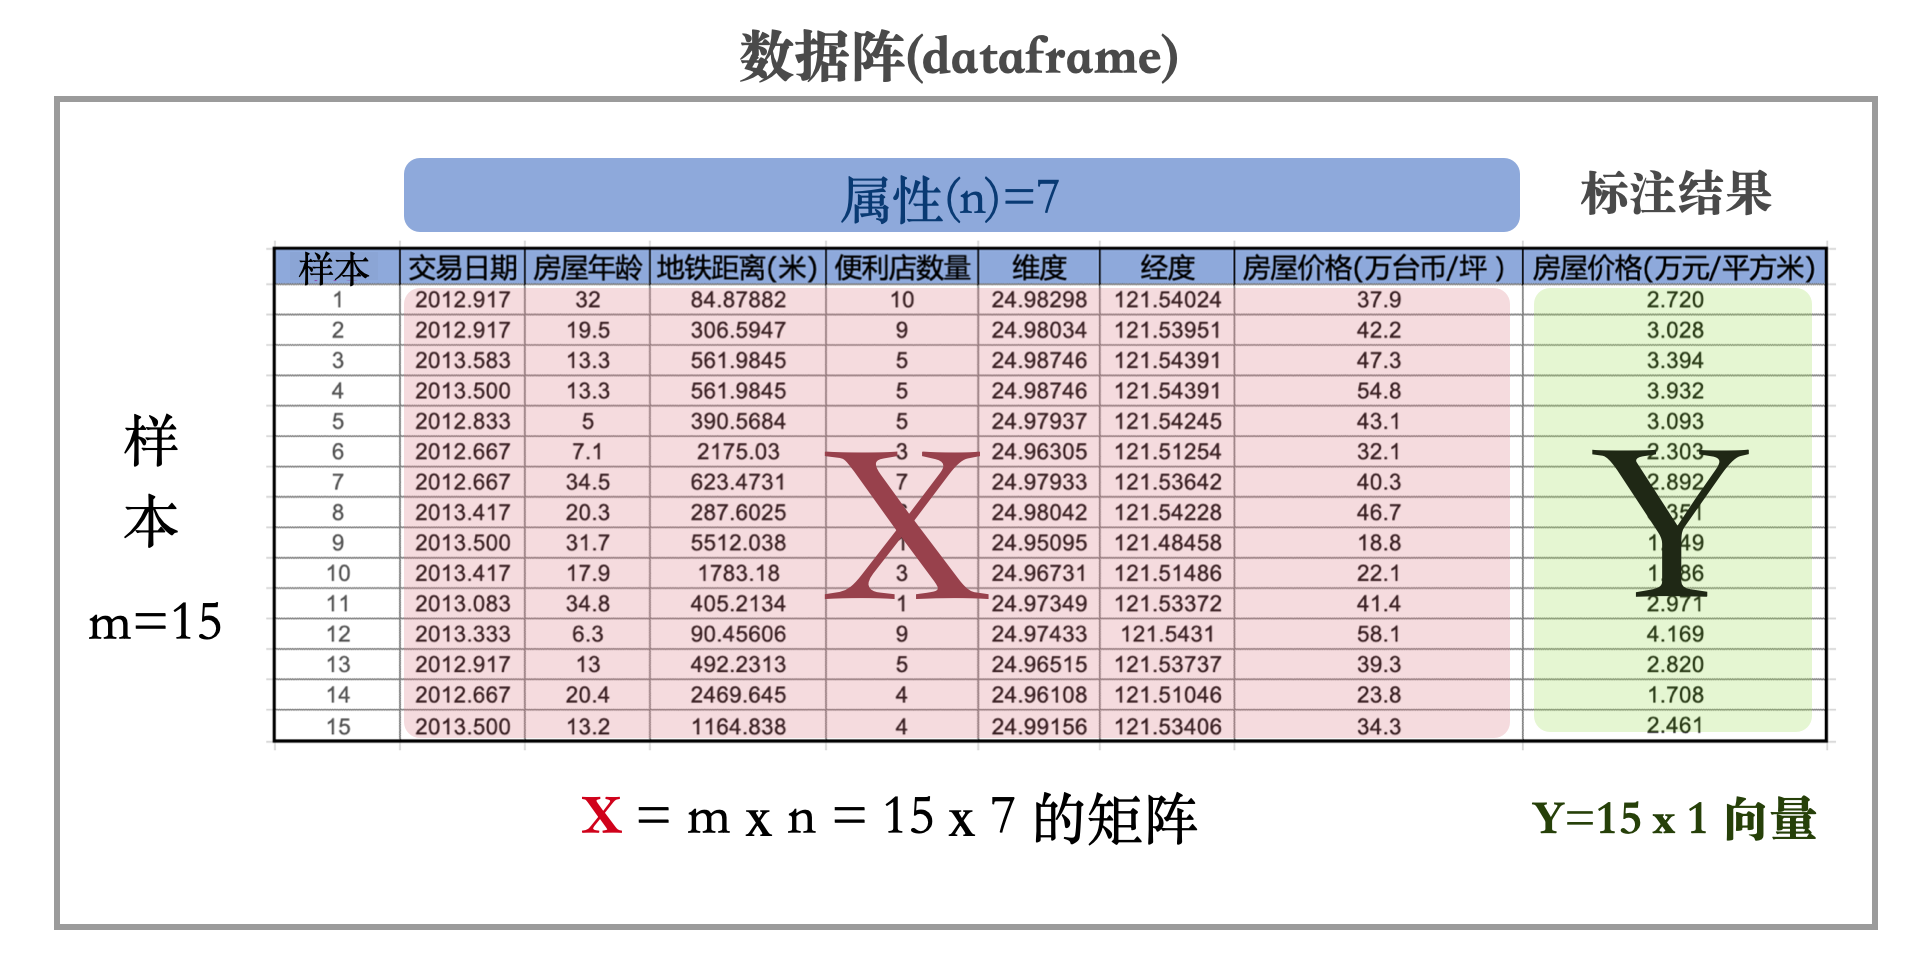
\includegraphics[width=\textwidth]{fig/dataframeVis}
\end{figure}
\begin{align*}
	\text{房屋价格} & = \beta_0 + \beta_1  \text{房屋年龄} + \beta_2 \text{地铁数量} + \cdots + \beta_7 \text{经度} 
\end{align*}
\end{frame}


\begin{frame}{问题回顾:线性回归详解}
线性回归:
\begin{itemize}
	\item 等式左边: 结果$y$, \underline{假设连续}
	\item 等式右边: 属性$\beta$($w$) 和 参数变量$X (m \times n)$, m 个样本,n 个属性
	\item 可视化: 一个\underline{结果轴}和\underline{多个属性轴}(n)
	\item 可视化: 最高到三维
\end{itemize}
\begin{figure}[H]
	\centering
	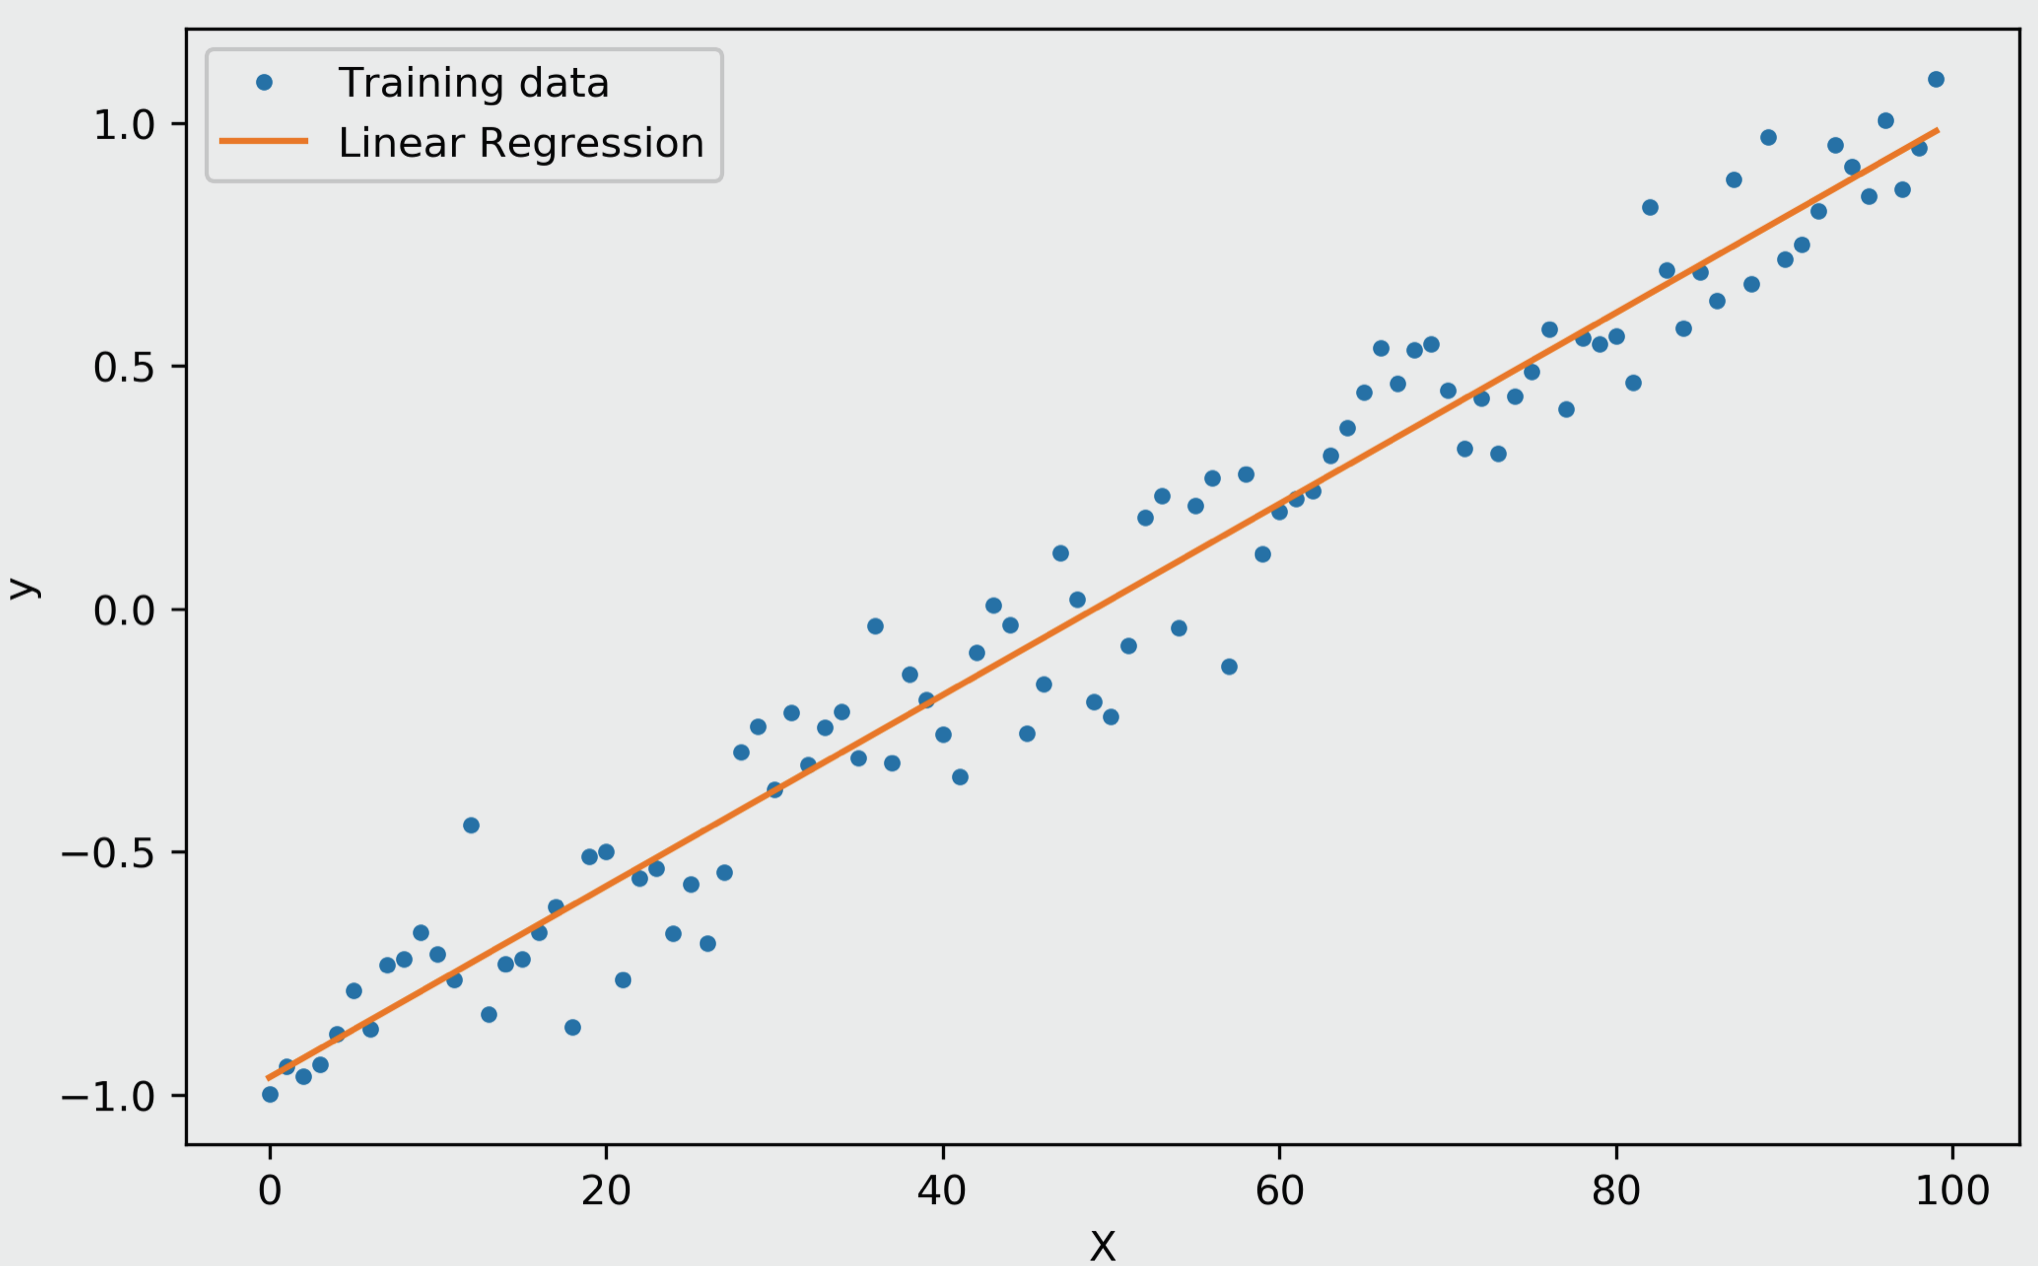
\includegraphics[width=0.7\textwidth]{fig/LinearReg}
\end{figure}
\end{frame}

\begin{frame}{问题回顾:线性回归详解}
三维图片:一个结果($Y$)轴,两个属性轴($x_1, x_2$)	
\begin{figure}[H]
	\centering
	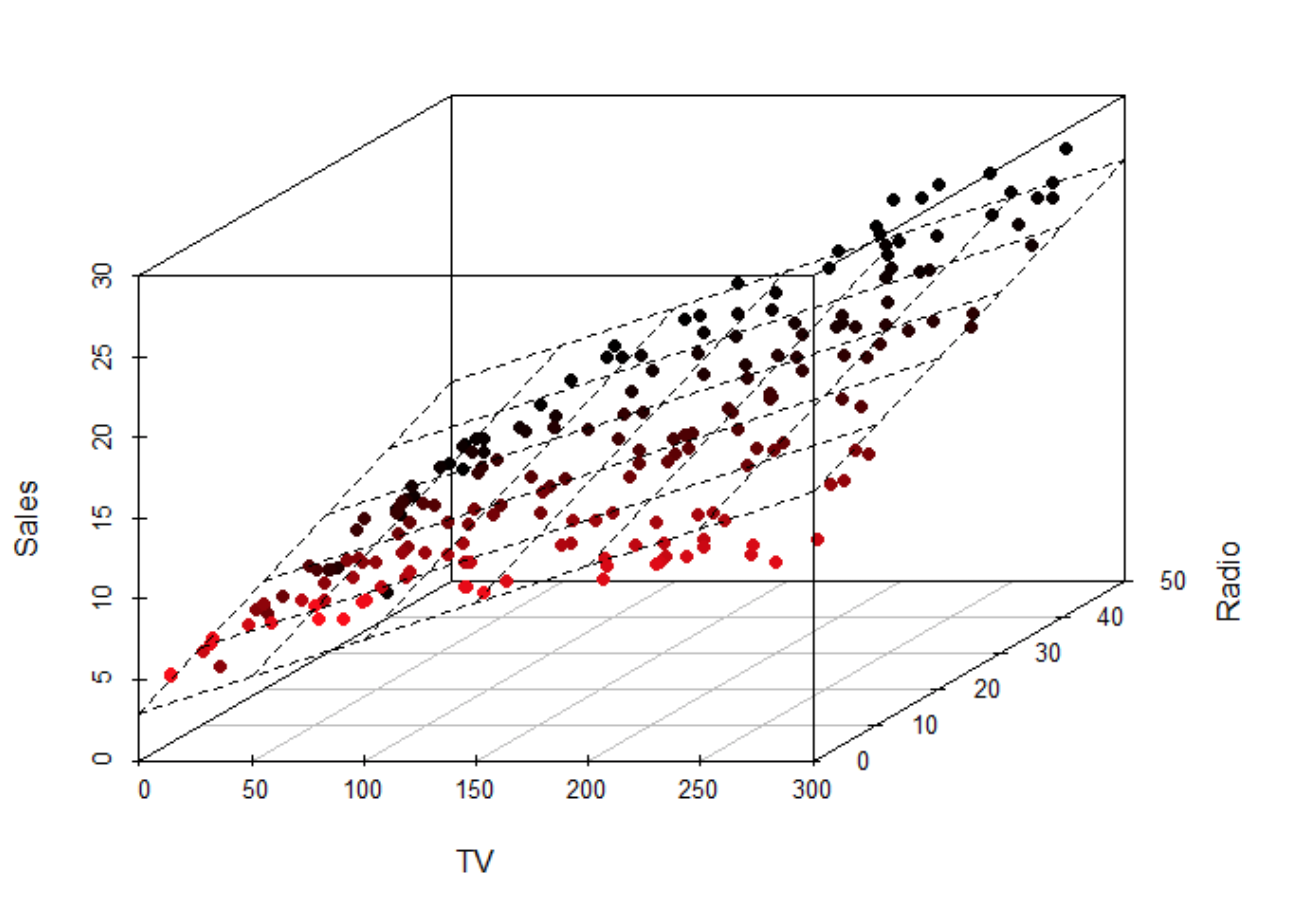
\includegraphics[width=0.9\textwidth]{fig/LinearReg3D}
\end{figure}
\end{frame}


\begin{frame}{从线性回归引入到分类}
	从线性回归切入到分类有两个角度:
	\setlength\itemsep{0.6em}
	\begin{itemize}
		\item 继续沿用线性回归思路: 
		\begin{itemize}
		\setlength\itemsep{0.3em}
		\item \underline{逻辑回归(Logistic Regression)}
		\item \underline{线性判别分析(Linear Discriminant Analysis, LDA)}
		\end{itemize}
		\item 抛弃线性回归思路,通过向量点积引入(试讲时会特别讲解)
	\end{itemize}
	
	\underline{教材的问题有}:
	\begin{itemize}
		\item 沿用了线性回归思路,但是并没有介绍逻辑回归(logistic regression)或者线性判别分析(LDA)
		\item 想要介绍分界面,但是没有把背后的数学点积问题讲清楚
	\end{itemize}
	
	\hfil
	
	什么意思? 请看下图!
\end{frame}

\begin{frame}{从线性回归引入到分类}
再看一下表格
		\begin{table}[H]
		\centering
		\begin{tabular}{lccc}
		\hline 
			属种 & 结果($y$) &花瓣长度 & 花瓣宽度 \\
			\hline 
			山鸢尾 & 0 & 1.4 & 0.2 \\
			山鸢尾 & 0 & 1.7 & 0.4 \\
			变色鸢尾 & 1 & 3.9  & 1.4 \\
			变色鸢尾 & 1& 4.9 & 1.5 \\
			维吉尼亚鸢尾 & 2 & 6.9 & 2.3  \\
			维吉尼亚鸢尾 & 2 & 6.1 & 1.9 \\
			\hline  
		\end{tabular}
\end{table}	
\end{frame}

\begin{frame}{从线性回归引入到分类}
\begin{figure}[H]
	\centering
	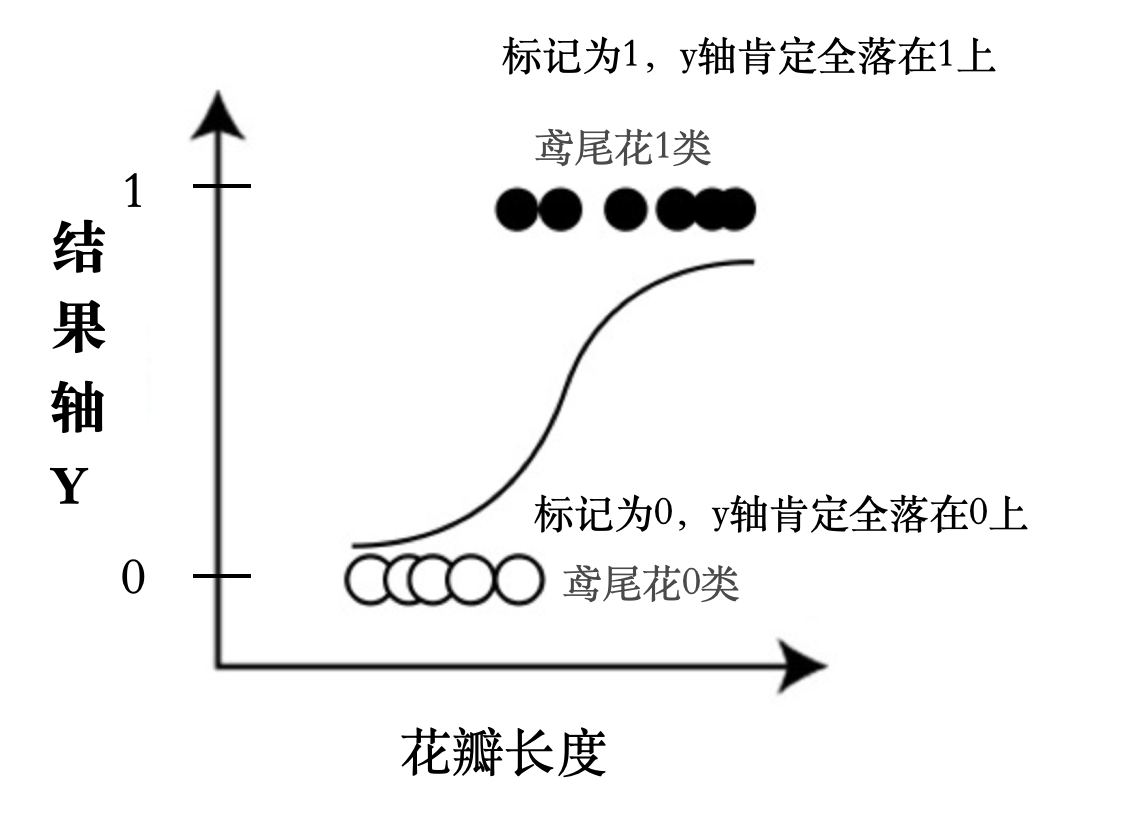
\includegraphics[width=0.9\textwidth]{fig/logisticreg1}
\end{figure}	
\end{frame}


\begin{frame}{从线性回归引入到分类}
\begin{figure}[H]
	\centering
	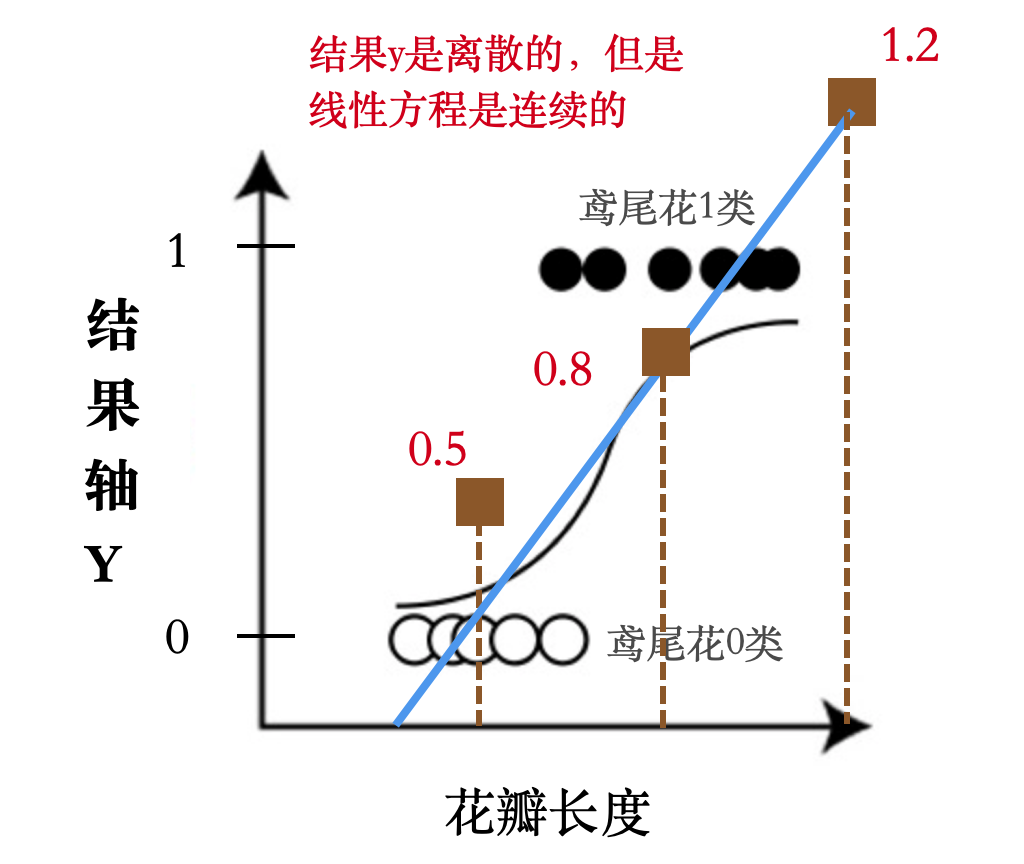
\includegraphics[width=0.9\textwidth]{fig/logisticreg2}
\end{figure}	
\end{frame}

\begin{frame}{从线性回归引入到分类}
引入逻辑回归(logistic regression), sigmoid function:
	\begin{align*}
		\sigma(z) = \frac{1}{1+e^{-z}} = \frac{1}{1+e^{X\beta + \varepsilon}}
	\end{align*}
	\begin{figure}[H]
		\centering
		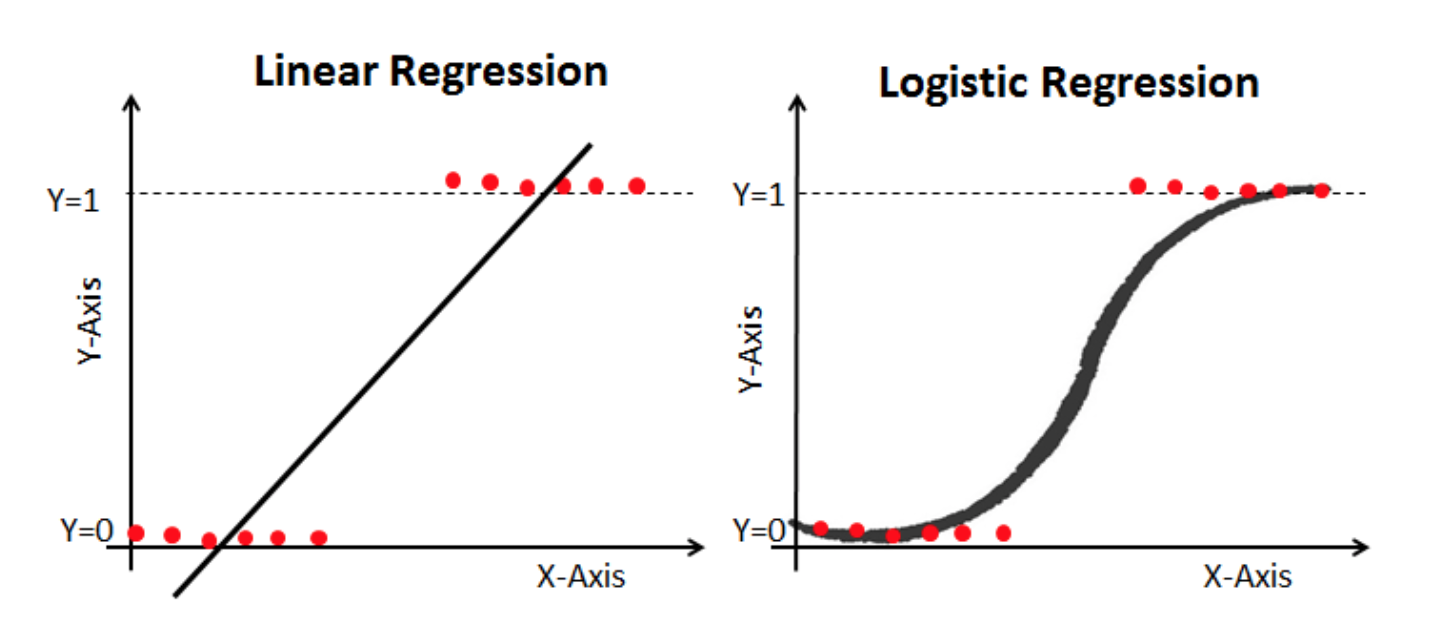
\includegraphics[width=0.9\textwidth]{fig/logisticreg3}
	\end{figure}
\end{frame}


\begin{frame}{从线性回归引入到分类}
我就不明白,怎么教材上分类的时候,$Y$轴上会出现一条\underline{斜线}呢?
\begin{figure}
	\centering
	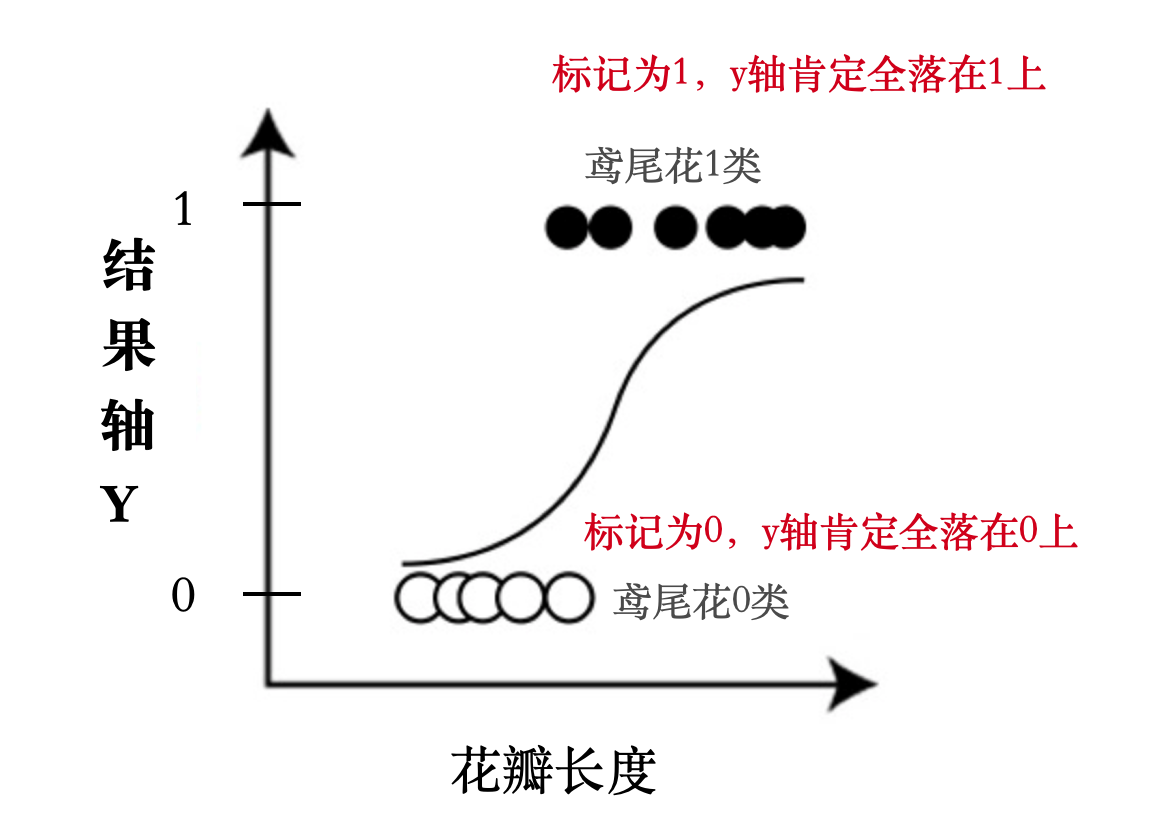
\includegraphics[width=0.8\textwidth]{fig/logisticreg4}
\end{figure}	
\end{frame}



\section{线性分类的切入方法再思考}

\begin{frame}{线性分类的切入}
	线性分类的切入:
	\begin{itemize}
	\setlength\itemsep{0.6em}
		\item 延续线性回归思路,需要转换$Y$轴,借助logistic regression(sigmoid function) 
		\item 不延续线性回顾思路,完全代数性质(点积)
	\end{itemize}
	\begin{align*}
		a \cdot b = ||a|| ||b|| \cos \theta
	\end{align*}
	\begin{figure}[H]
		\centering
		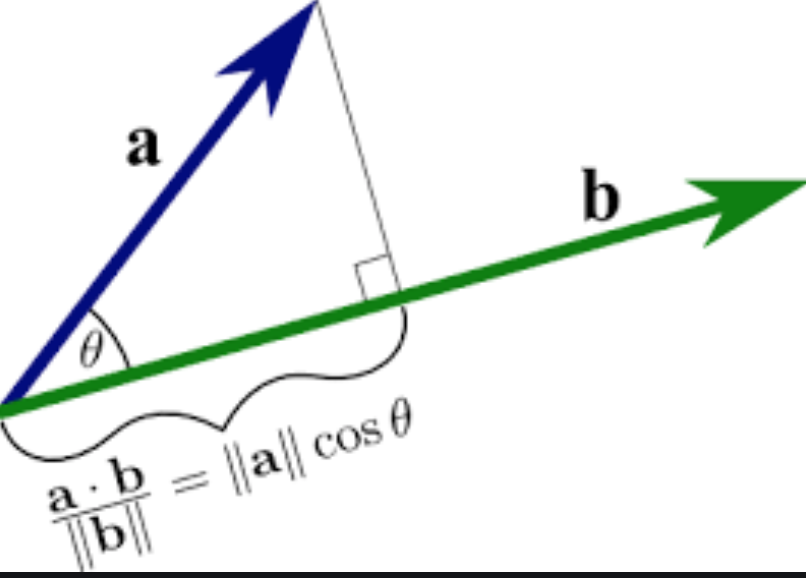
\includegraphics[width=0.5\textwidth]{fig/C2C2svmprojc}
	\end{figure}
\end{frame}

\begin{frame}{线性分类的切入}
Vladimir Vapnik 还活着,所以可以了解到最初他是如何创立支持向量机(Support vector machine)的。
\begin{columns}
\begin{column}{0.3\textwidth}
\centering
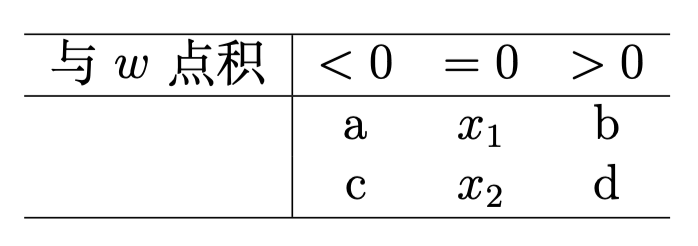
\includegraphics[width=\textwidth]{fig/P2dotpTable}
\end{column}
\begin{column}{0.7\textwidth}
	\begin{figure}[H]
	\centering
	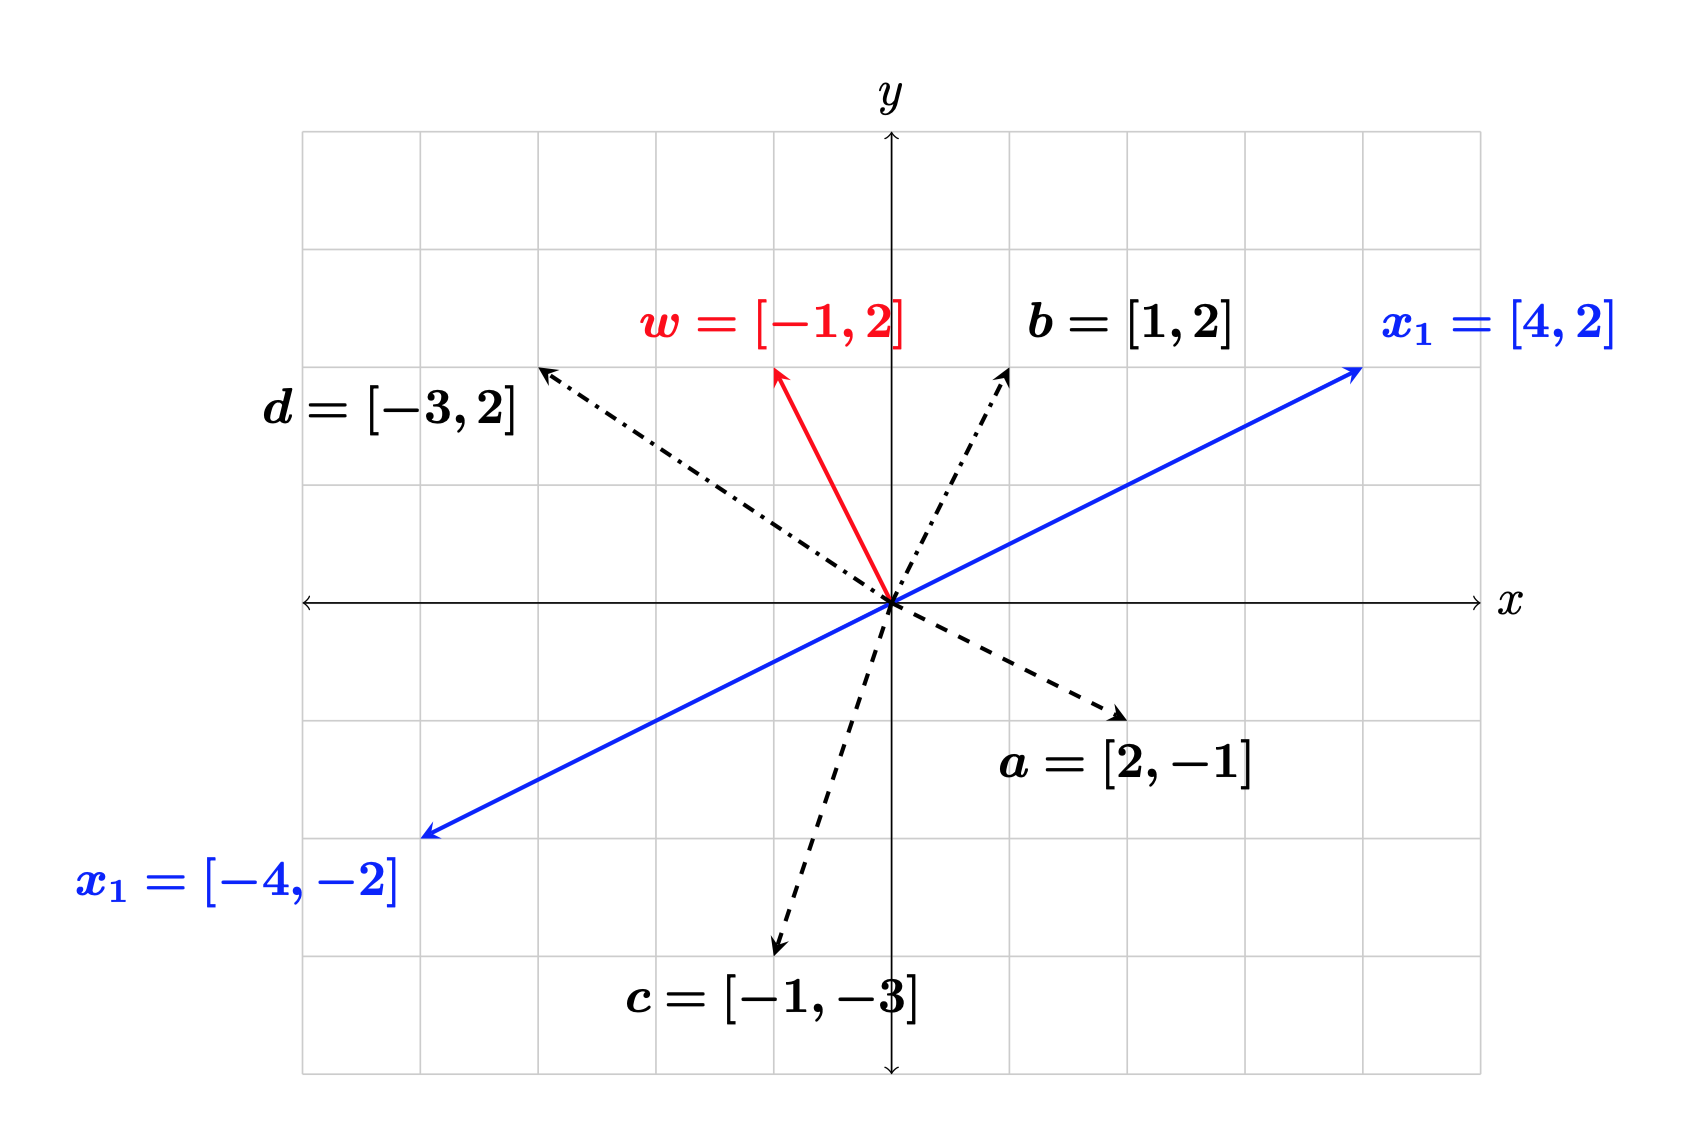
\includegraphics[width=\textwidth]{fig/C2C2dotprodt}
\end{figure}	
\end{column}
\end{columns}
Reference: Patrick Winston (Youtube, 点击率1百万)
\end{frame}

\newcommand{\notimplies}{\;\not\!\!\implies}

\begin{frame}{高中教材}
	高中教材36页,下列公式的错误:
	\begin{align*}
		\gamma = \min \gamma^{i} \notimplies   \min \frac{2}{\gamma}
	\end{align*}
	应该为
	\begin{align*}
		\gamma = \max \gamma^{i}  \ \Rightarrow \ \min \frac{2}{\gamma}
	\end{align*}
\begin{figure}[H]
	\centering
	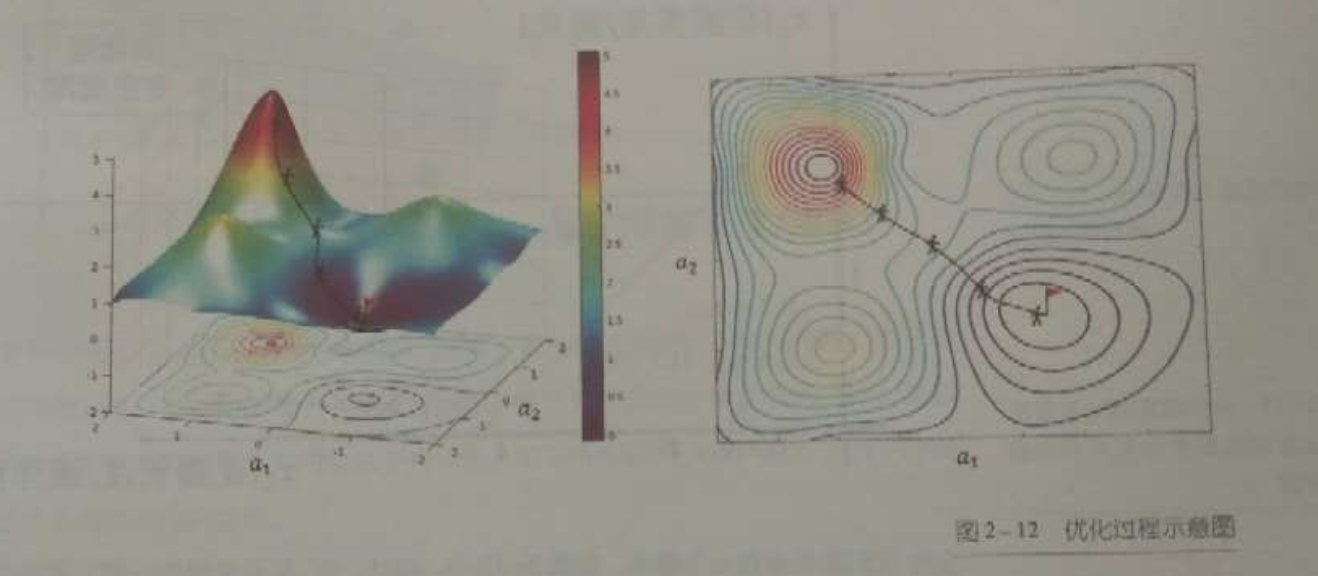
\includegraphics[width=0.6\textwidth]{fig/textbookGD}
\end{figure}
\end{frame}



\section{详解梯度下降法和其动画演示}

\begin{frame}{梯度下降法: 为什么?}
	天不生仲尼(牛顿),亘古如长夜;求极限值(最大值,最小值)
	\begin{itemize}
	\setlength\itemsep{0.6em}
		\item 笨办法, 遍历$[1, 5, 8, 9]$;
		\item 设置方程,求导 (一阶条件,二阶条件);
		\item 但是计算机不会求导(需要人求导后,告诉它公式)
		\item 而且计算机不会解方程: \begin{itemize}
		\setlength\itemsep{0.3em}
		\item 极限值位置,遍历?
		\item 有规律的找到极限值, 随机找一个点,然后迭代逼近优化值
		\end{itemize}
	\end{itemize}
	最小化损失函数(损失越小,预测越准确):
	\begin{align*}
		L = \min_{w, b} f(w, b) 
	\end{align*}
	我们关心什么?
	\begin{itemize}
		\item \underline{是什么$w$值},让$L$最小
	\end{itemize}
\end{frame}

\begin{frame}{梯度下降法原理}
	机器学习中,梯度下降法(Gradient Descent)的公式可能是最为常见的公式之一了:
	\begin{align*}
		w_{t+1} = w_t - \alpha f'(x) 
	\end{align*}
	\begin{itemize}
		\item $\alpha$ learning rate(更新参数/速率)
		\item $f'(x)$为损失函数$f(w, b)$的导数
		\item 算法: 随机取一个$w$,然后逼近优化值。
	\end{itemize}
	我们就通过下面的例子和动画来理解下梯度下降法的原理。虽然具体的损失函数可能不同,但是原理是一致的,我们用一个最简单的例子来说明:
	\begin{align*}
		f(x) & = x^2-2x-3 \\
		f'(x) & = 2x - 2
	\end{align*}
\end{frame}


\begin{frame}{梯度下降法原理}
当方程处于极限值时,导数等于0: 极限值左右两边,导数正负值相反。
\begin{figure}[H]
	\centering
	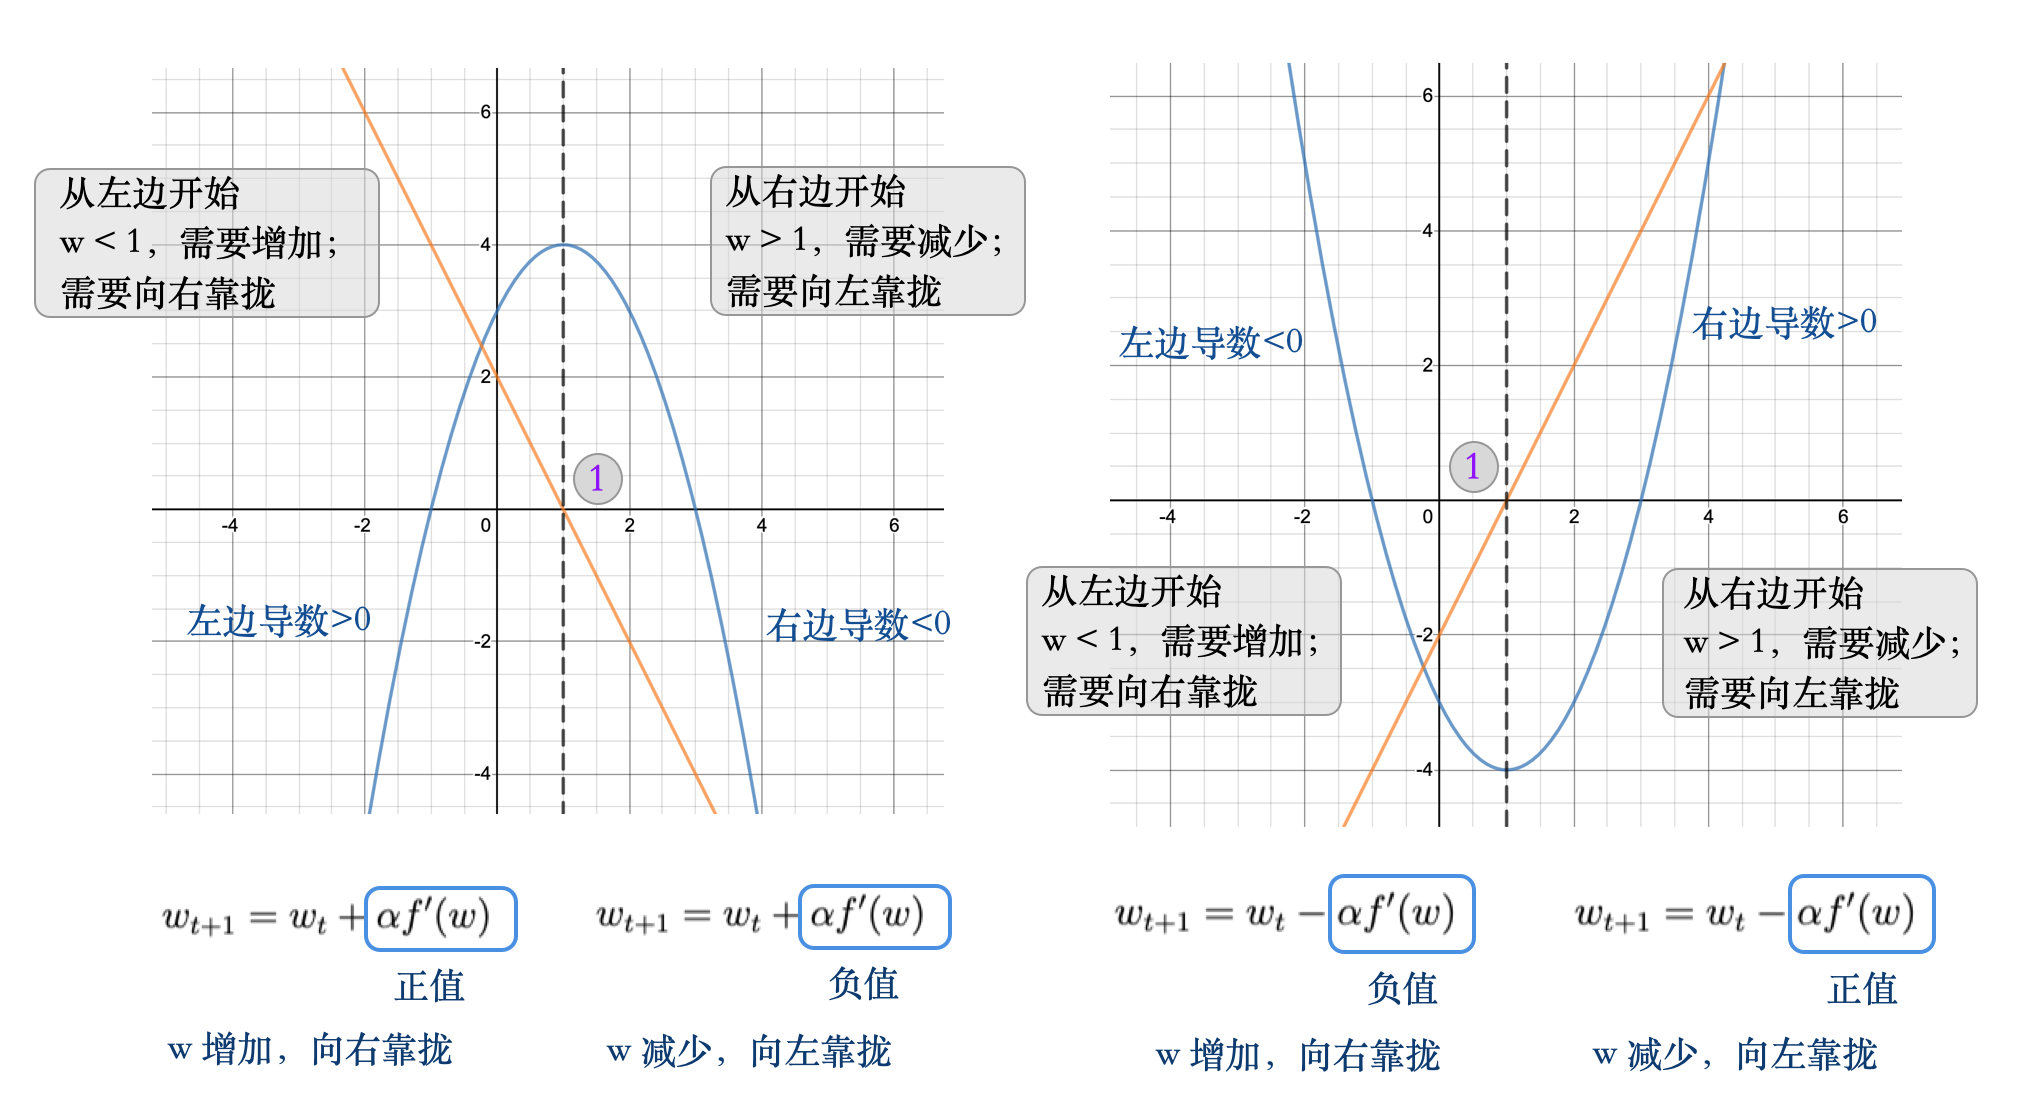
\includegraphics[width=0.96\textwidth]{fig/C2C2GradientDes}
\end{figure}		
\end{frame}

\begin{frame}{梯度下降法原理}
\begin{align*}
	& w_{t+1} = w_t - \alpha f'(w) \\
	& \text{$w$ 增加,向右靠拢}
\end{align*}	
\begin{figure}[H]
	\centering
	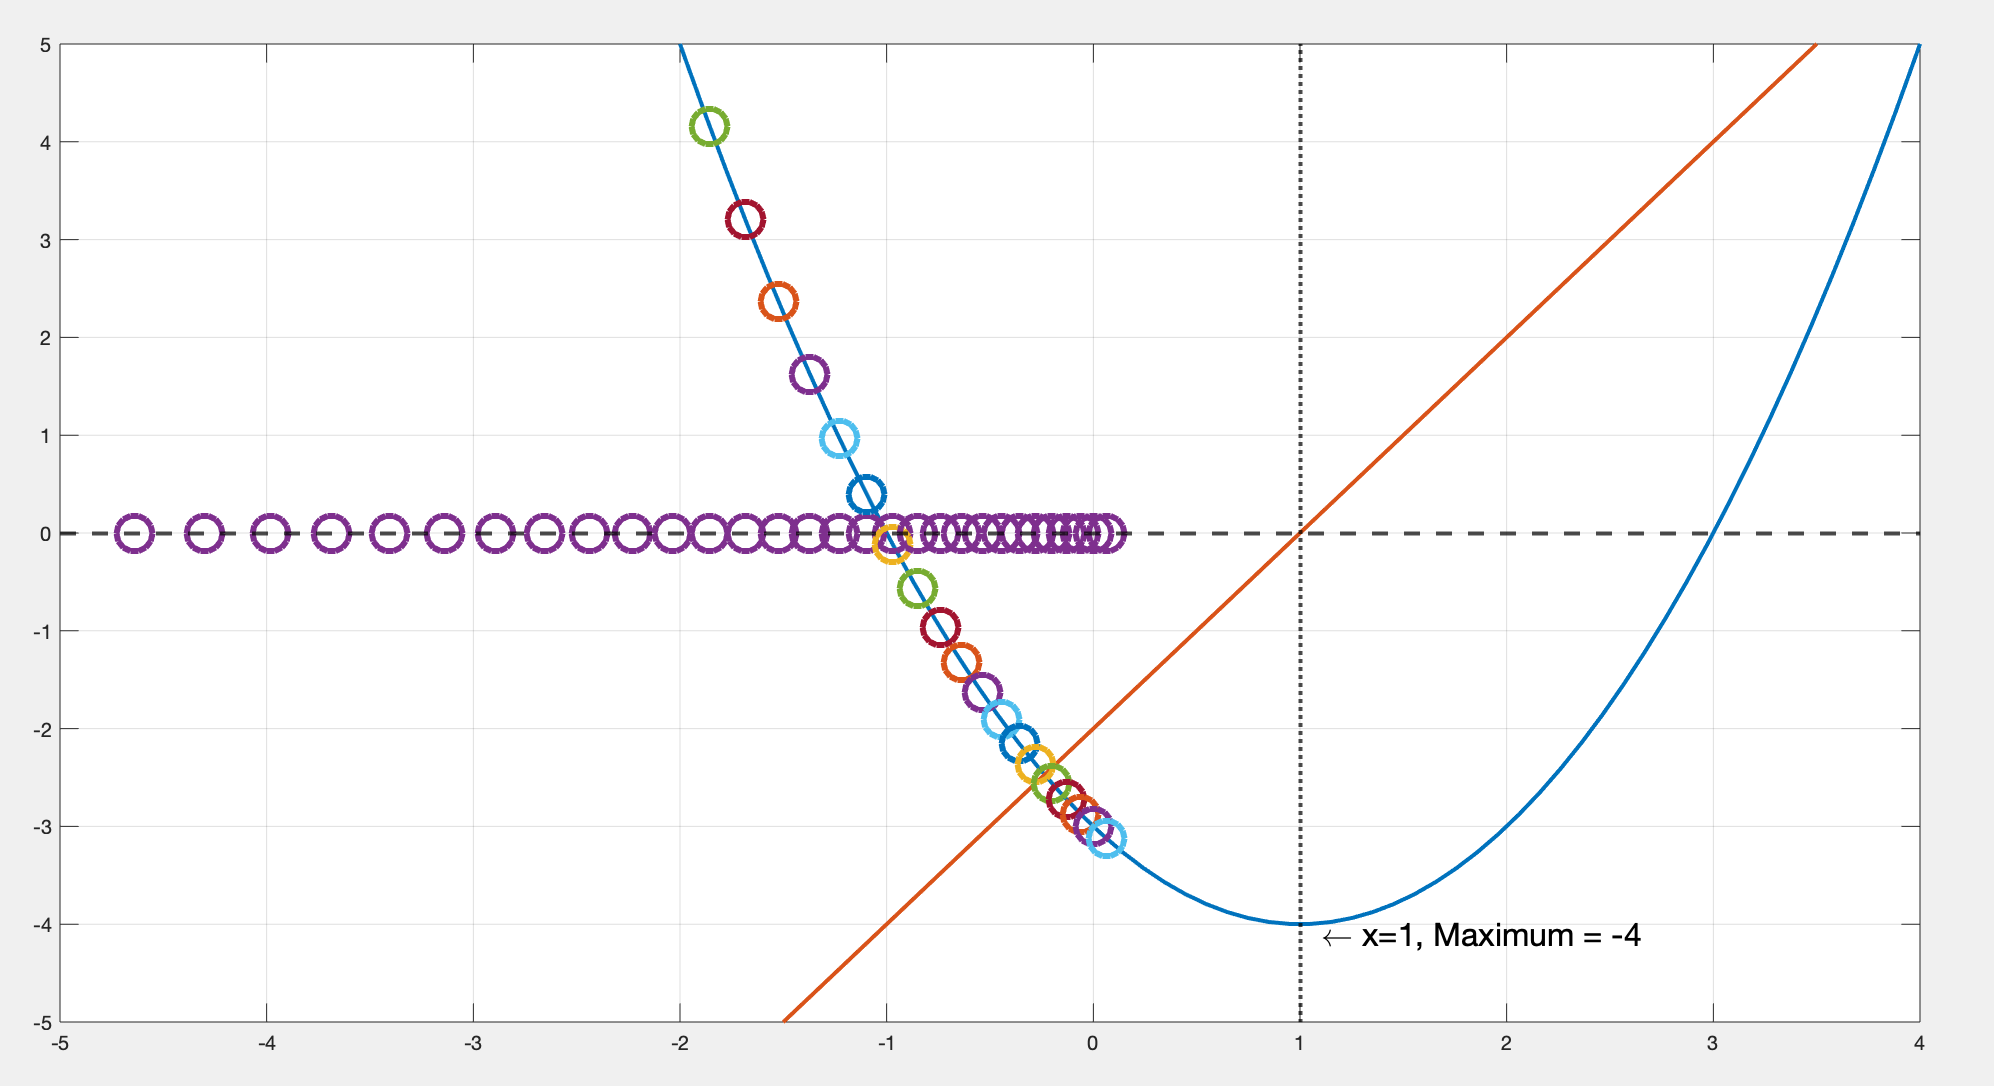
\includegraphics[width=0.8\textwidth]{fig/GDani1}
\end{figure}
\end{frame}


\begin{frame}{梯度下降法原理}
\begin{align*}
	& w_{t+1} = w_t - \alpha f'(w) \\
	& \text{$w$ 减少,向左靠拢}
\end{align*}	
\begin{figure}[H]
	\centering
	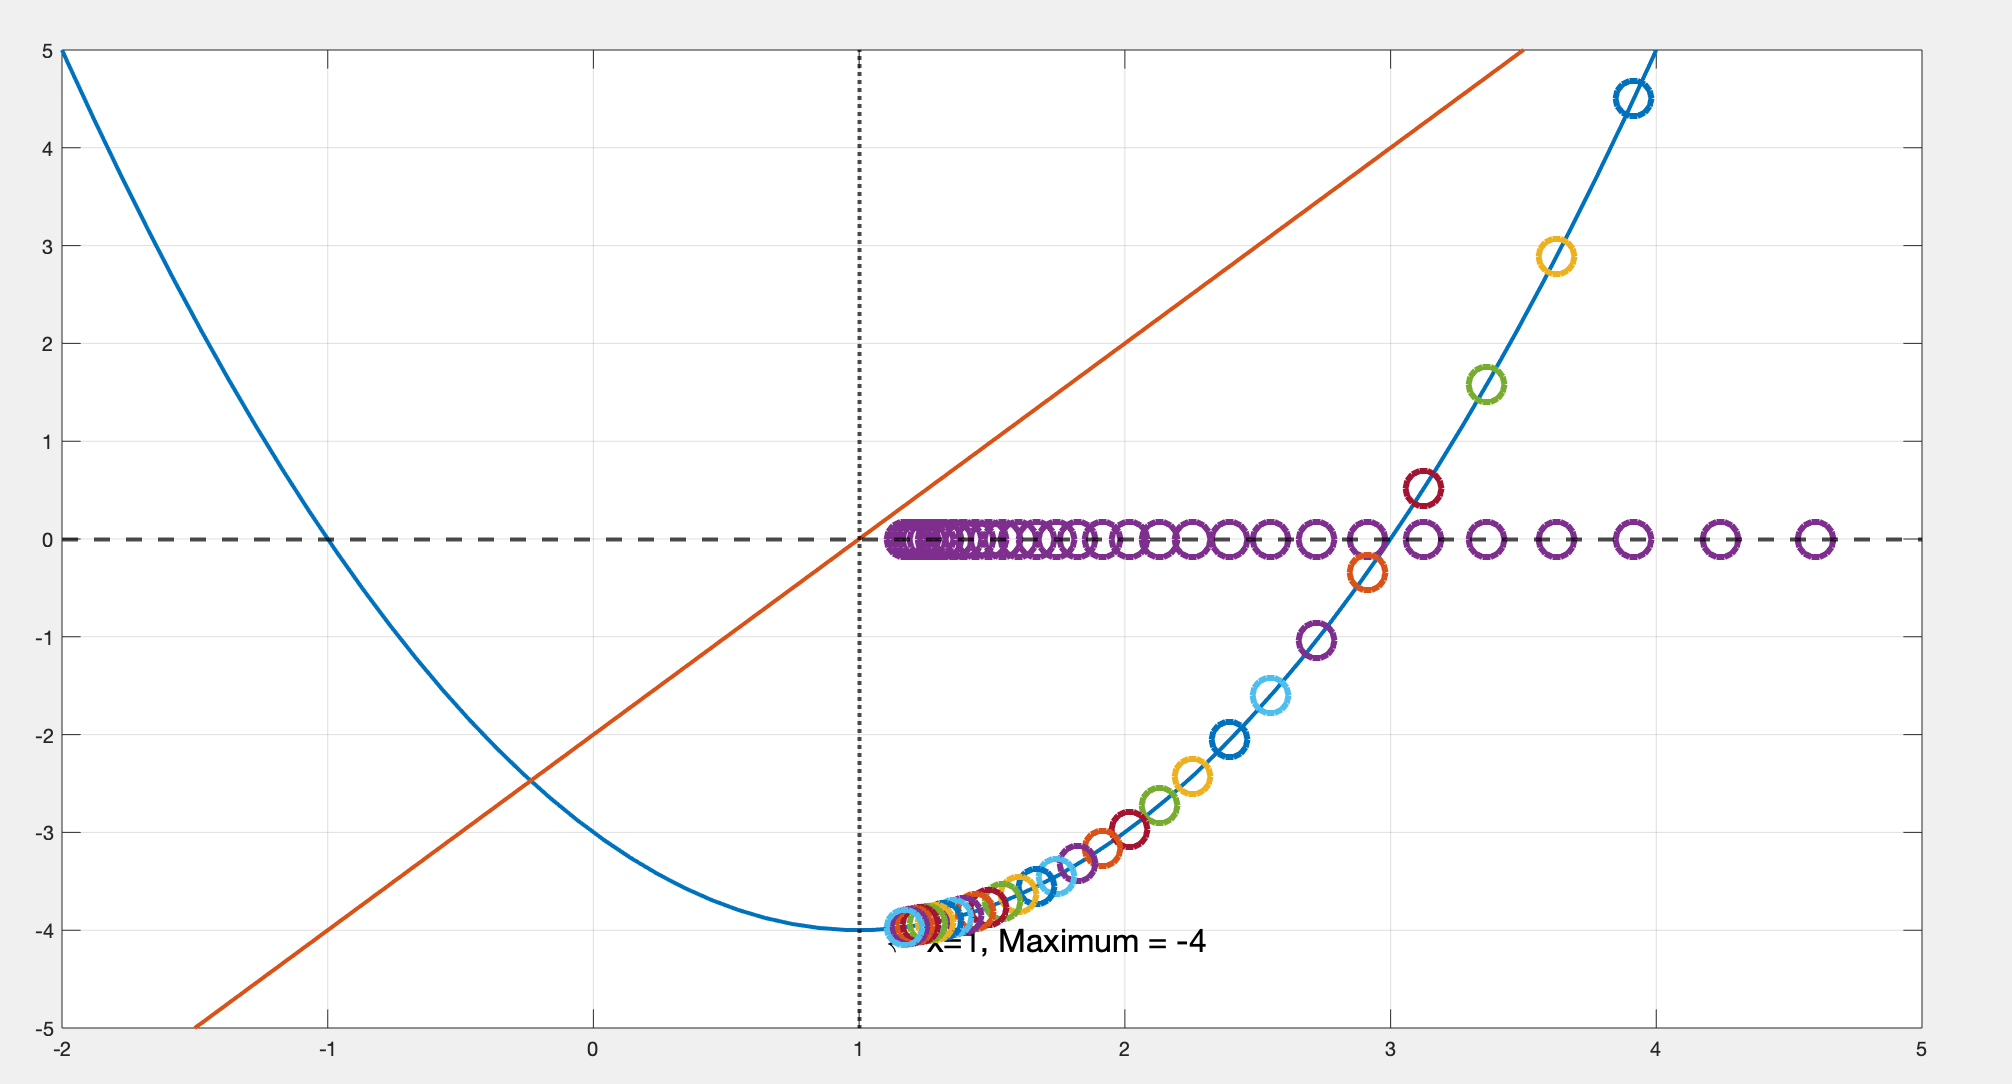
\includegraphics[width=0.8\textwidth]{fig/GDani2}
\end{figure}
\end{frame}

\begin{frame}{梯度下降法原理: 动画}
	下面我们看一下梯度下降法的动画!请注意:
	\begin{itemize}
	\setlength\itemsep{0.6em}
		\item 计算机是看不到\underline{我们看到的图形的}
		\item 计算机只认识公式:$w_{t+1} = w_t - \alpha f'(w)$
		\item 计算机也搞不懂你为什么让它计算这些东西,更不清楚为什么要迭代30次或者50次,也不明白$\alpha$选大选小的影响
		\item 两个大脑论
	\end{itemize}
	\begin{figure}[H]
	\centering
	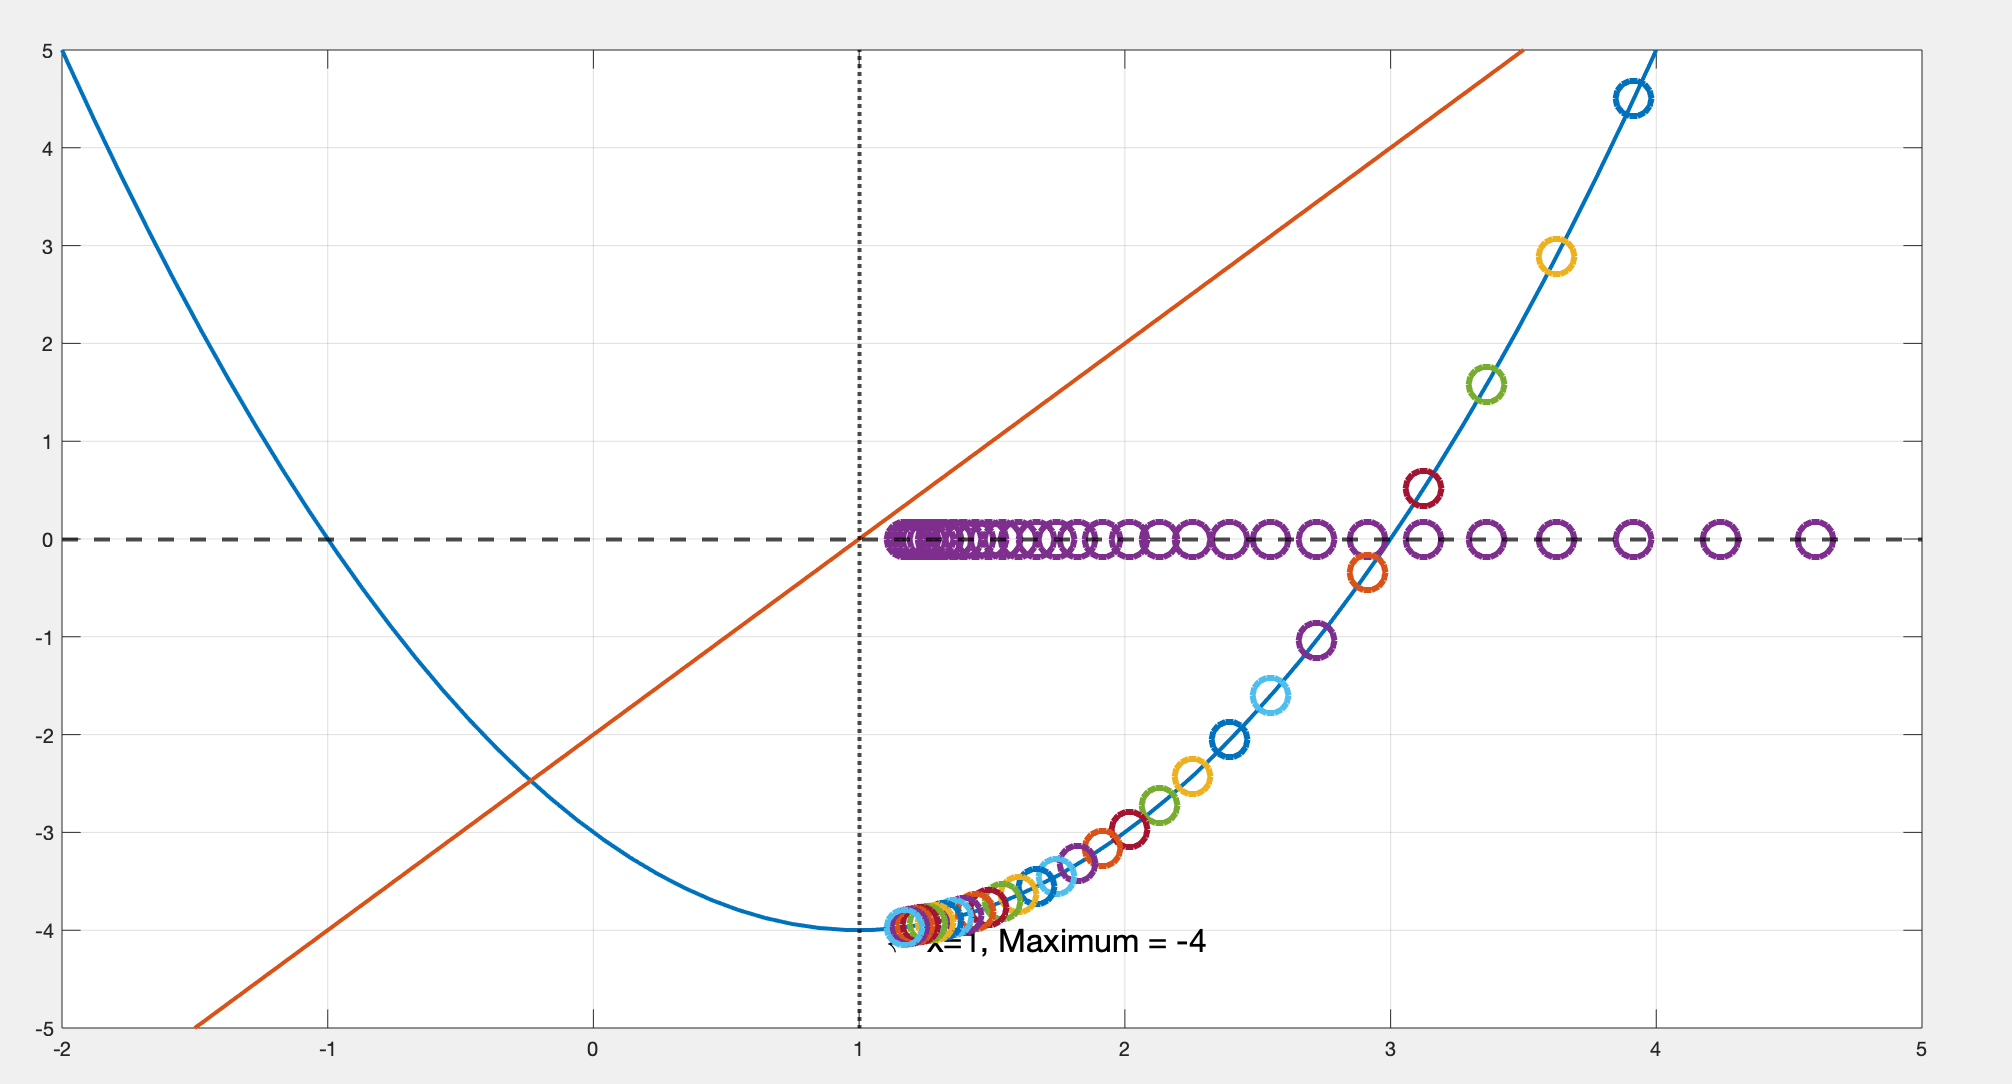
\includegraphics[width=0.6\textwidth]{fig/GDani2}
\end{figure}
\end{frame}


\begin{frame}{结语}
	因为平时大家都很忙,各自有自己的项目和工作,有些想法不好集中沟通的,我觉得大家都可以做成视频:
	\begin{itemize}
	\setlength\itemsep{0.6em}
		\item 超越时空来共享想法
		\item 有助于系统梳理思路
		\item 而且非常有助于提供反馈
		\item \underline{答案全在网上,问题却在心中, 需要得是`时代在召唤'}
		\item 问题比答案更重要!
		\item How many roads must a man walk down before you call him a man?
		\item The answer, my friend, is blowing in the wind
	\end{itemize}
\end{frame}























\end{document}